Las medidas realizadas así como los cálculos requeridos podemos visualizarlos en la tabla (\ref{table_exp}). Para la determinación de la tensión superficial se ha aplicado la ecuación (\ref{eq_nouy}) con el radio del anillo $r = 9.75$mm. Como es de esperar la tensión superficial disminuye a medidas que aumentamos la temperatura.

Podemos comparar nuestro resultado frente al valor teórico $\sigma_t = 72\cdot 10^{-3}$N/m a una temperatura de 25ªC. Las condiciones ambientales en nuestro laboratorio eran de 22ºC, lo que significa que hemos obtenido un resultado inferior al valor teórico. A pesar de tener un error relativo del 1\% nuestra incertidumbre no abarcó en rango al valor teórico.

En la tabla (\ref{table_exp}) también se encuentran los resultados para $\sigma V_{m}^{2/3}$, datos que representamos en la figura (\ref{figure_eotvos}) frente a la temperatura medida, donde hemos considerado $V_m = 18 cm^3 \cdot mol^{-1}$. Con un ajuste por mínimos cuadrados podemos verificar la ecuación (\ref{eq_eotvos}) y determinar la constante de Eötvös $k$ como la pendiente de la recta. En este caso obtenemos $k = (2.8 \pm 0.3) \cdot 10^{-7} J/K \cdot mol^{2/3}$, valor superior al correspondiente según la literatura $k_t = 2.1 \cdot 10^{-7} J/K \cdot mol^{2/3}$.

A partir del término independiente podemos determinar también el valor de la temperatura crítica $T_k$. Manipulando la ecuación (\ref{eq_eotvos}) identificamos $T_k = \frac{b}{k}$ siendo $b$ el término independiente de nuestro ajuste. Así pues, obtenemos $T_k = 456 \pm 12$K, valor muy por debajo de los $T_{kt} = 647$K correspondientes al agua (siendo la diferencia de entorno al 30\%).

\begin{figure}[t]
	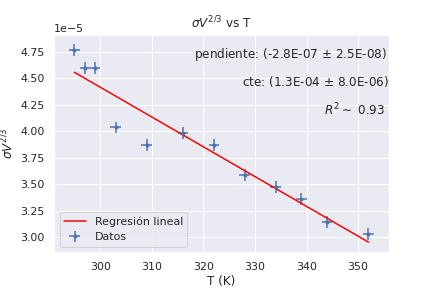
\includegraphics[width=\linewidth]{eotvos}
	\caption{Representación $\sigma V_{m}^{2/3}$ frente a la temperatura.}
	\label{figure_eotvos}
\end{figure}